\documentclass{article}


\usepackage{arxiv}
\rhead{\scshape Technical Report - \today}

\usepackage[utf8]{inputenc} % allow utf-8 input
\usepackage[T1]{fontenc}    % use 8-bit T1 fonts
\usepackage{hyperref}       % hyperlinks
\usepackage{url}            % simple URL typesetting
\usepackage{booktabs}       % professional-quality tables
\usepackage{amsfonts}       % blackboard math symbols
\usepackage{amsmath}        % math environments
\usepackage{nicefrac}       % compact symbols for 1/2, etc.
\usepackage{microtype}      % microtypography
\usepackage{graphicx}
\usepackage{xcolor}
\usepackage{tikz}
\usepackage{float}
\graphicspath{ {./images/} {../images/} }


\title{Fine-Tuning Qwen3-VL-2B for ASL to English Translation%
  \thanks{Code and full report available at
  \href{https://github.com/mamounyosef/sign-language-bridge}{github.com/mamounyosef/sign-language-bridge}.}}


\author{
 Ma'moun Yosef \\
  Department of Artificial Intelligence \\
  University of Jordan \\
  Amman, Jordan \\
  \texttt{mam0233493@ju.edu.jo} \\
}


\begin{document}
\maketitle

\begin{abstract}
This report describes an end-to-end pipeline for translating continuous
American Sign Language (ASL) video into English text by fine-tuning the
$2$-billion-parameter \emph{Qwen3-VL-2B-Instruct} vision and language
model. The training recipe combines a multi-tier LoRA / RSLoRA adaptation
with per-tier learning rates and gradient-clipping budgets, a two-corpus
staged schedule that pretrains on OpenASL before fine-tuning on How2Sign,
a preprocessing pipeline of pose-guided signer cropping, CLAHE contrast
enhancement, and pre-extracted MediaPipe landmark overlays, and an InfoNCE
auxiliary loss anchoring the pooled vision embedding to its caption
embedding. On a custom $90/5/5$ stratified split, the trained model
produces fluent English in the register of the target captions and often
captures the meaning of the signed input, but the word-level overlap with
references is modest (test BLEU-$4 = 1.64$, ROUGE-L $= 10.43$ on the
How2Sign test partition). The methodological caveats that bound this
result are stated in detail. The report's contribution is a transparent
engineering account rather than a state-of-the-art claim.
\end{abstract}


% \keywords{Sign language translation \and Vision--language models \and Qwen3-VL \and
% LoRA \and Curriculum learning \and InfoNCE}


\section{Introduction}
\label{sec:introduction}

Sign languages are full natural languages, expressed through coordinated
movement of the hands, face, and upper body. They are a primary means of
communication for a substantial fraction of the more than $430$ million
people worldwide estimated by the World Health Organization to live with
disabling hearing loss~\cite{who2026deafness}. Outside the Deaf community,
signed messages usually rely on a human interpreter to reach a wider
audience. Automatic sign language translation aims to narrow this gap by
mapping recorded signing directly to text in a target language. The task
addressed here is \emph{continuous} American Sign Language (ASL) to English
translation: given a video clip of a signer producing one or more full
sentences, the system must produce the corresponding English text.

The task is much harder than spoken-language machine translation. The input
is a video stream rather than a sequence of discrete tokens, so timing and
meaning have to be inferred together. ASL also carries meaning through
several channels at once, including facial expression and body posture, any
of which can change the sense of a manual sign. Sign boundaries are not
marked explicitly, public corpora are small by the standards of modern
language modeling, and pretrained video-capable models are trained mostly
on natural imagery, not on the close-range, fast-motion footage typical of
signing.

This report describes the third of three attempts at the problem. The
first two prototypes used custom vision front ends (MediaPipe landmarks,
then a pretrained CNN) feeding an MLP, a Transformer encoder, and a
pretrained LLM decoder with all components trainable; neither produced
coherent translations. The current attempt replaces that pipeline with a
single pretrained model that natively accepts video,
\emph{Qwen3-VL-2B-Instruct}, fine-tuned end-to-end with a recipe that fits
the available compute. The recipe combines a multi-tier LoRA / RSLoRA
adaptation, a two-corpus staged schedule (OpenASL then How2Sign), an
easy-first curriculum within each stage, and a preprocessing pipeline that
crops the signer, enhances contrast with CLAHE, and overlays pre-extracted
MediaPipe landmarks on the input frames. No state-of-the-art claim is
made; the data splits were built locally rather than taken from the
released splits, and the consequences for comparability are discussed in
Section~\ref{sec:limitations}.


\section{Background: Parameter-Efficient Adaptation}
\label{sec:background}
Full fine-tuning of a 2-billion-parameter vision and language model is
impractical on a single GPU, so the adaptation in this work is restricted to a
small set of trainable parameters using Low-Rank Adaptation
(LoRA)~\cite{hu2022lora}. LoRA freezes the pretrained weights and inserts a
trainable update of the form $\Delta W = B A$ alongside each adapted linear
layer, where $A$ and $B$ are low-rank matrices of rank
$r \ll \min(d_\mathrm{in}, d_\mathrm{out})$. Only $A$ and $B$ are updated
during training, which reduces the number of trainable parameters by orders of
magnitude relative to full fine-tuning while leaving the inference graph
unchanged once the update is merged.

At training time the update is scaled by a factor $\alpha / r$. As shown by
Kalajdzievski~\cite{kalajdzievski2023rslora}, this scaling causes the effective
learning rate to shrink as $r$ grows, which limits the benefit of increasing
the rank. Rank-stabilized LoRA (RSLoRA) replaces the factor with
$\alpha / \sqrt{r}$, which separates the effective learning rate from $r$ and
allows the rank to be tuned per layer without retuning the learning rate.
RSLoRA is used throughout this work; the per-layer ranks chosen for the vision
encoder, the language model, the output head, and the auxiliary contrastive
head are specified in Section~\ref{sec:training}.


\section{Datasets}
\label{sec:datasets}

Two corpora of paired ASL video and English text are used in this work:
How2Sign~\cite{duarte2021how2sign} and OpenASL~\cite{shi2022openasl}. They
differ markedly in domain, size, and caption quality, and are used at different
stages of training (Section~\ref{sec:training}).

\subsection{How2Sign}
\label{sec:data-how2sign}

How2Sign~\cite{duarte2021how2sign} is a multi-view ASL corpus of roughly 80
hours of "How To" instructional content with manually verified English
transcripts. Its captions are short, well-formed sentences, and the recording
conditions are comparatively controlled, with a limited set of signers and
consistent framing. In this work How2Sign serves as the higher-quality
fine-tuning corpus.

\subsection{OpenASL}
\label{sec:data-openasl}

OpenASL~\cite{shi2022openasl} is a roughly 300-hour open-domain corpus
collected from online ASL video, with English captions taken from existing
subtitle tracks. The captions are noisier than How2Sign's, including
occasional ASR-style errors, and the material covers a broader range of
register, topic, signer identity, and recording quality. OpenASL serves as the
larger but noisier pretraining corpus.

\subsection{Duration Filtering and Custom Splits}
\label{sec:data-splits}

A duration filter restricts both corpora to clips between $1.3$ and $8$
seconds. The choice is motivated by the intended deployment scenario: the
model is expected to run in near-real-time on short windows of incoming
signing, on the order of a few seconds at a time, so training on clips
longer than the typical inference window would not reflect the system's
actual operating regime. Shorter clips, in turn, frequently contain only
fragments of signing. After filtering, a combined pool of $51{,}499$ clips
remains, of which $32{,}628$ ($63.4\%$) come from OpenASL and $18{,}871$
($36.6\%$) from How2Sign.

The official released splits of How2Sign and OpenASL were not preserved.
Several cleaning passes were applied to both corpora before splitting:
exact-duplicate removal, cross-split data-leakage removal, a words-per-second
filter dropping rows with $\mathrm{word\_count} / \mathrm{duration\_sec} > 5.0$
(implausibly fast captions), and fuzzy near-duplicate removal applied both
within and across the original splits. In addition, a set of eight light
text-normalisation passes was applied to all captions, covering steps such as
stripping non-ASCII characters, normalising smart quotes and dashes to ASCII
equivalents, collapsing repeated punctuation, sentence-casing all-caps text,
and dropping rows with no alphabetic content. The cleaning passes left the
original per-split sizes unbalanced across the two sources, so the cleaned
data was pooled and a single stratified 90/5/5 random split was applied to
the combined pool, stratified by source so that each split preserves the
$63.4\%$/$36.6\%$ source ratio.
The resulting train, validation, and test sets contain $46{,}349$, $2{,}575$,
and $2{,}575$ clips respectively, with $59.74$ hours of training video in
total. Per-source counts are summarised in Table~\ref{tab:dataset-splits}.

\begin{table}[h]
\centering
\caption{Final stratified 90/5/5 splits after the 1.3-to-8-second duration
filter. Column percentages are within-source; the overall train/val/test
split is $90.0\%/5.0\%/5.0\%$ for both sources.}
\label{tab:dataset-splits}
\begin{tabular}{l r r r r}
\toprule
Source     & Total      & Train      & Val      & Test     \\
\midrule
How2Sign   & $18{,}871$ & $16{,}983$ & $944$    & $944$    \\
OpenASL    & $32{,}628$ & $29{,}366$ & $1{,}631$& $1{,}631$\\
\midrule
Combined   & $51{,}499$ & $46{,}349$ & $2{,}575$& $2{,}575$\\
\bottomrule
\end{tabular}
\end{table}

\begin{figure}[h]
  \centering
  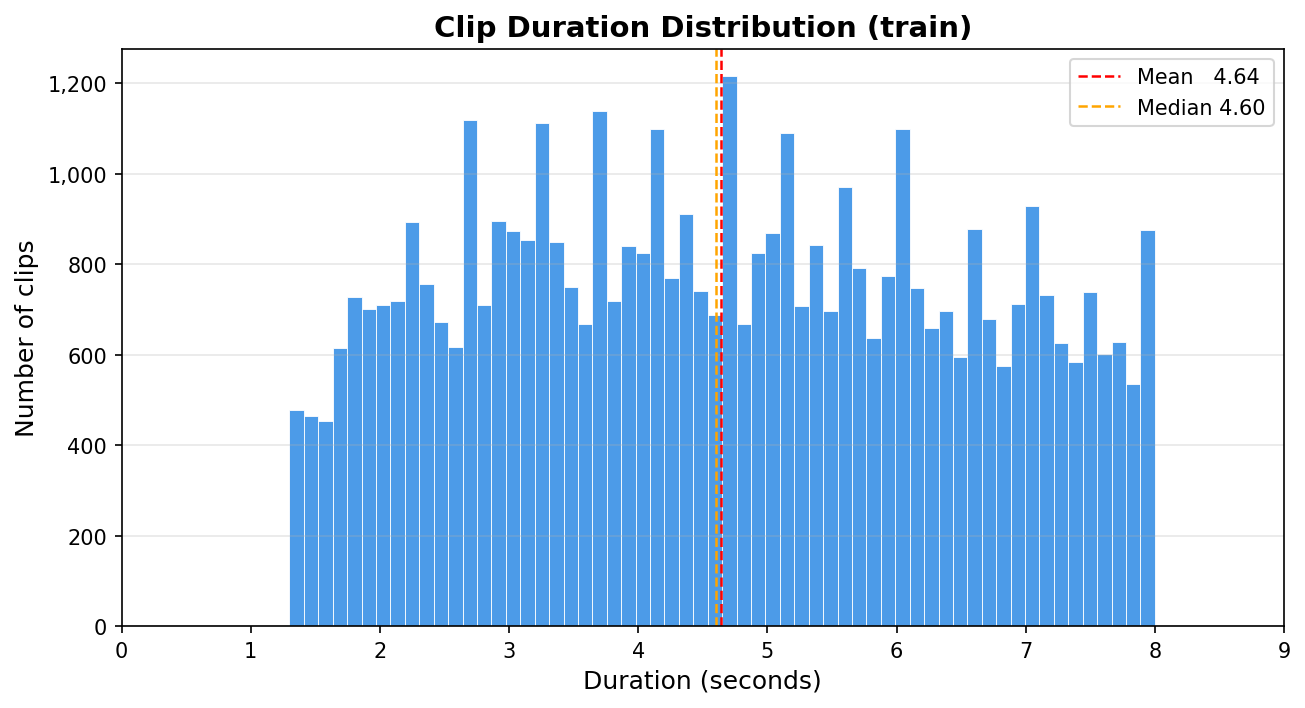
\includegraphics[width=0.48\linewidth]{clip_duration_distribution.png}\hfill
  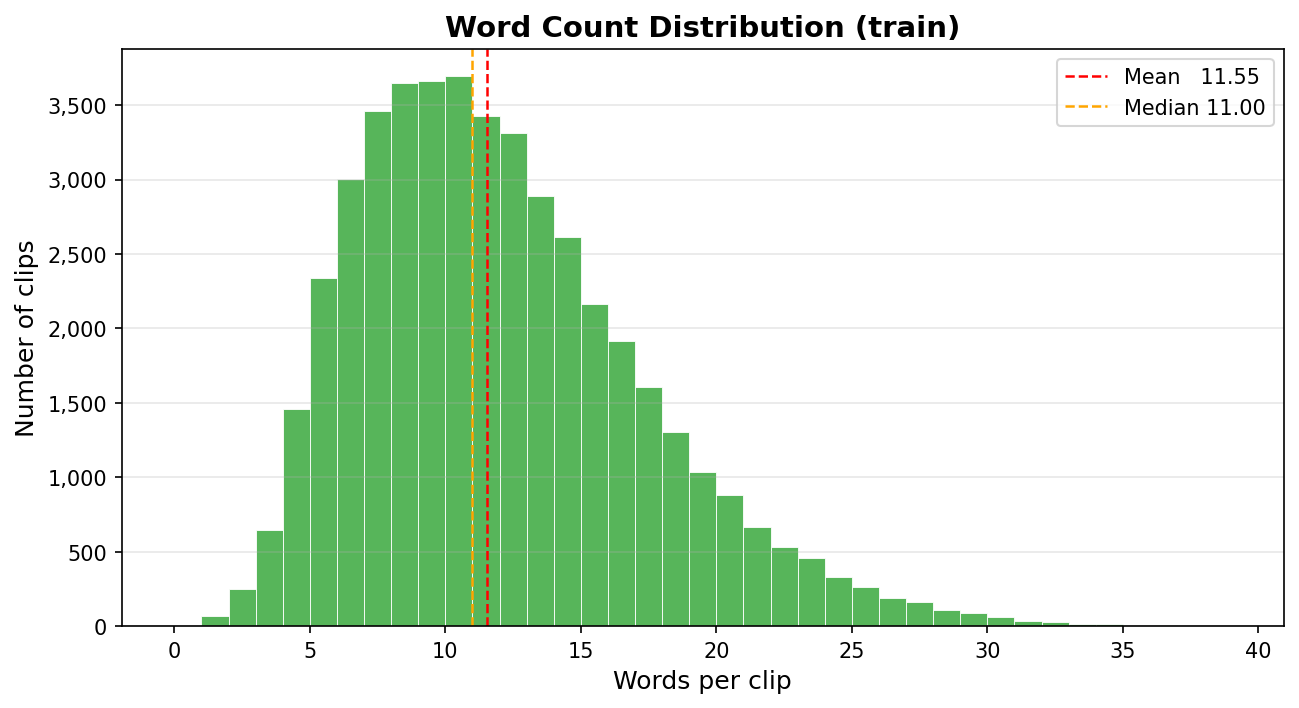
\includegraphics[width=0.48\linewidth]{word_count_distribution.png}
  \caption{Distributions over the combined cleaned pool. Left: clip duration
  in seconds, restricted to the $1.3$-to-$8$-second filter window. Right:
  caption word count.}
  \label{fig:dataset-distributions}
\end{figure}


\section{Data Preprocessing Pipeline}
\label{sec:preprocessing}

Every clip is passed through a fixed sequence of per-frame transforms. Three
always-on visual stages are applied in order, illustrated in
Figure~\ref{fig:preprocessing-stages}, followed by a stochastic augmentation
suite that is active only during training. The frame rate and the per-frame-pair
pixel budget are set per source. OpenASL clips are decoded at $18$ frames per
second with a maximum of $150 \times 32 \times 32 \approx 392 \times 392$
pixels per frame pair, while How2Sign clips are decoded at $20$ frames per
second with a maximum of $180 \times 32 \times 32 \approx 429 \times 429$
pixels per frame pair. A clip-level cap of $20{,}480 \times 32 \times 32$
pixels across all frames is also enforced.

\subsection{Signer Cropping}
\label{sec:pre-crop}

A single static bounding box per clip is used to crop each frame to the
signing region before any further processing. The bounding boxes are
computed offline using MediaPipe pose detection and stored alongside the
dataset. Cropping before the Qwen3-VL processor's internal resize ensures
that the pixel budget lands on the signer rather than on background.

\subsection{CLAHE Contrast Enhancement}
\label{sec:pre-clahe}

Contrast-Limited Adaptive Histogram Equalisation (CLAHE) is applied to every
cropped frame. The frame is converted to LAB colour space, CLAHE with a clip
limit of $2.0$ and an $8 \times 8$ tile grid is applied to the L channel, and
the result is converted back to RGB. Operating on the L channel preserves hue
while enhancing local contrast, which makes hand outlines and finger
separations easier to read under the varied lighting conditions seen across
the two corpora.

\subsection{Landmark Overlay}
\label{sec:pre-landmarks}

After CLAHE, a skeleton-like overlay of pre-extracted MediaPipe landmarks is
drawn on every frame. Each clip carries $21$ keypoints per hand and $6$
upper-body joints (shoulders, elbows, and wrists), with anatomically connected
keypoints joined by thin line segments. The left hand, the right hand, and the
upper-body skeleton are drawn in distinct colours so that the vision encoder
receives an explicit structural cue alongside the underlying imagery, which is
particularly useful on lower-resolution or motion-blurred frames.

\subsection{Training-Time Augmentation}
\label{sec:pre-aug}

A stochastic augmentation suite is applied only at training time, after the
three always-on stages. The active augmentations are temporal jitter (small
frame shifts with edge replication), affine perturbation (a few degrees of
rotation, a few percent of translation, mild zoom), colour jitter (small
brightness, contrast, saturation, and hue swings), random grayscale, and
speed perturbation (resampling the frame sequence to simulate slightly slower
signing). Augmentation is disabled during the first epoch of each training
phase and turned on from the second epoch onward (so that the model can see each original dataset in full at least one time); full parameter values are
listed in Appendix~\ref{app:augmentation}.

\begin{figure}[h]
  \centering
  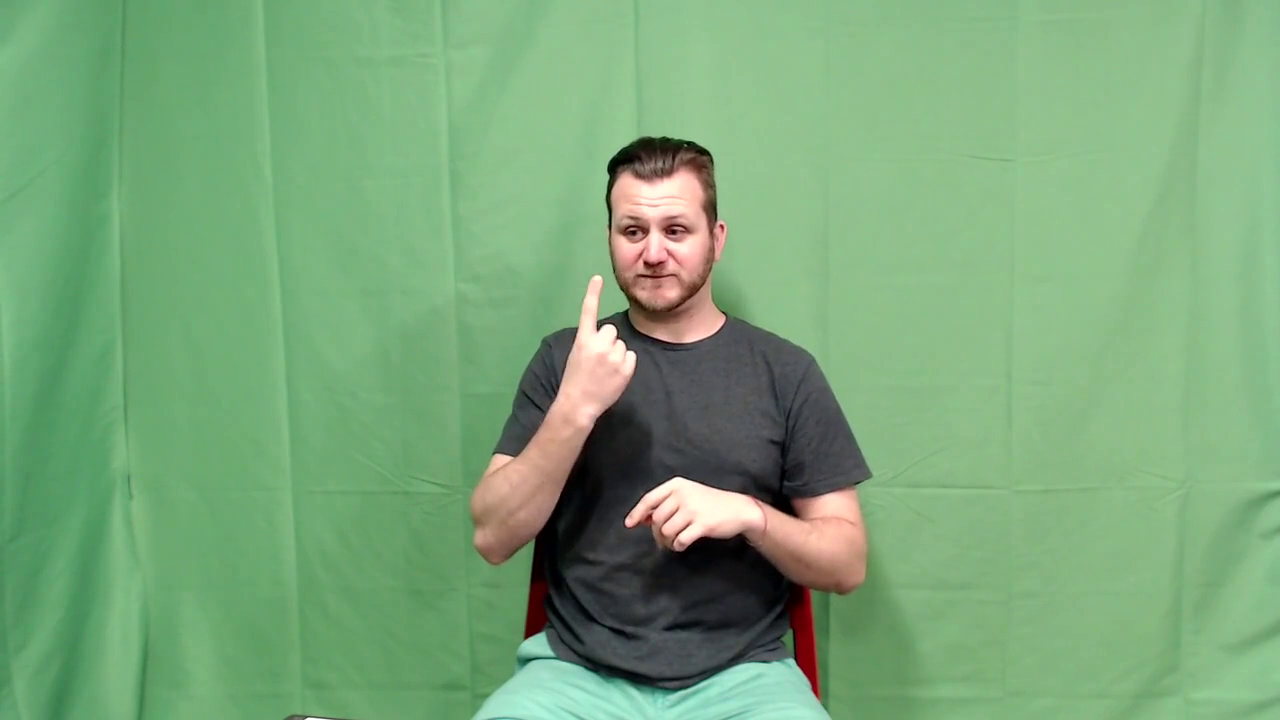
\includegraphics[width=0.24\linewidth]{raw.png}\hfill
  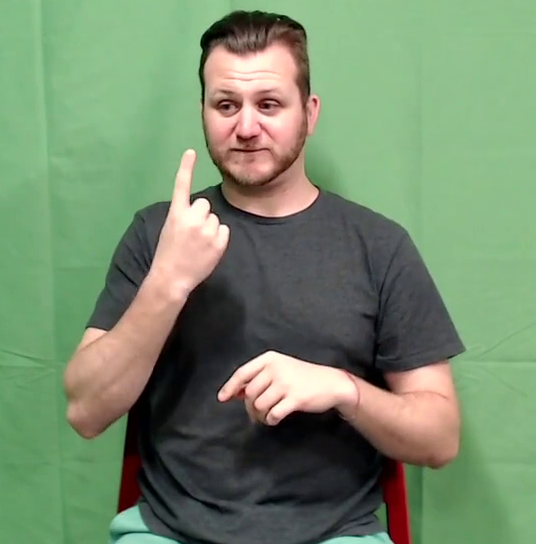
\includegraphics[width=0.24\linewidth]{cropped.png}\hfill
  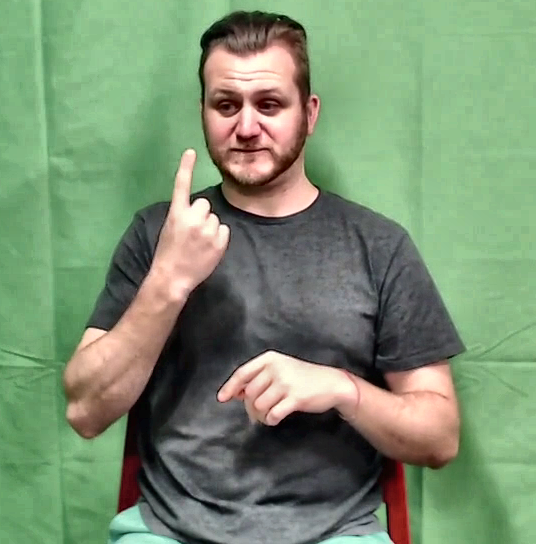
\includegraphics[width=0.24\linewidth]{clahe.png}\hfill
  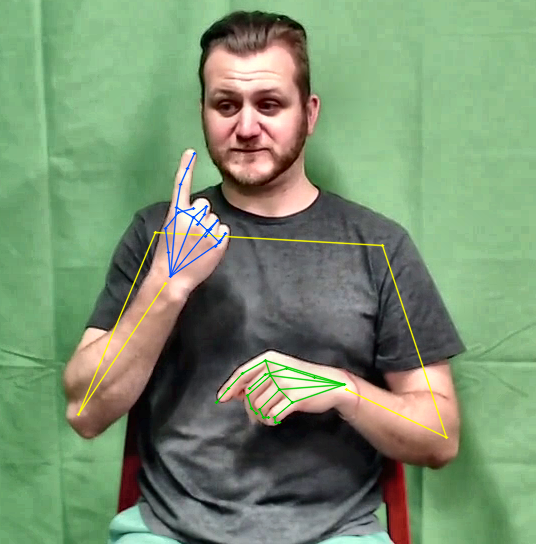
\includegraphics[width=0.24\linewidth]{landmark_overlay.png}
  \caption{Always-on preprocessing stages applied to every clip. From left to
  right: raw decoded frame; after signer cropping using the precomputed
  MediaPipe pose bounding box; after CLAHE contrast enhancement on the L
  channel of LAB; after the MediaPipe landmark overlay ($21$ keypoints per
  hand plus $6$ upper-body joints).}
  \label{fig:preprocessing-stages}
\end{figure}


\section{Model Architecture}
\label{sec:architecture}

The model used in this work is the Qwen3-VL-2B-Instruct
backbone~\cite{qwen3vl2025} augmented by two small linear projection heads
added on top to support an auxiliary contrastive loss. All other components
are inherited from the released checkpoint.

\subsection{Qwen3-VL-2B Backbone}
\label{sec:arch-backbone}

The backbone consists of a vision tower coupled to a decoder-only language
model via a small connector. The vision tower is a 24-layer Transformer with
hidden size $1024$, $16$ attention heads, and an intermediate MLP size of
$4096$. Frames enter the tower through a three-dimensional patch embedding
(Conv3d) with spatial patch size $16$ and temporal patch size $2$, so each
visual token corresponds to a $16 \times 16$ pixel region pooled across two
consecutive frames. The tower's $1024$-dimensional outputs are projected to
the $2048$-dimensional language-model embedding space by a Patch Merger
module. In addition, three DeepStack mergers extract features from
vision-tower layers $5$, $11$, and $17$ and inject them into the language
stream alongside the final merger output, giving the language model
multi-scale access to the visual input.

The language model is a 28-layer Qwen3-architecture decoder with hidden size
$2048$, intermediate size $6144$, $16$ query heads, $8$ key-value heads
(grouped-query attention), and tied input and output embeddings over a
vocabulary of $151{,}936$ tokens. Multimodal Rotary Positional Embeddings
(M-RoPE) are used so that the same positional encoding handles text and video
tokens consistently. The total backbone parameter count is approximately
$2$ billion.

\subsection{InfoNCE Projection Heads}
\label{sec:arch-infonce-heads}

Two small linear projection heads are added on top of the released checkpoint,
mapping the pooled vision and text representations into a shared
$256$-dimensional embedding space for the InfoNCE contrastive loss described
in Section~\ref{sec:training}. Each head is a single bias-enabled linear
layer of shape $2048 \to 256$, initialised with a normal distribution of
standard deviation $0.02$. The heads are trained from scratch alongside the
LoRA adapters, and their weights are saved and restored separately at
checkpoint time.


\section{Training Methodology}
\label{sec:training}

The training recipe combines four components: a multi-tier LoRA adaptation
that splits the trainable parameters across the vision tower, the language
model, the output head, and the InfoNCE projection heads
(Section~\ref{sec:train-tiers}); a two-corpus staged schedule that pretrains
on OpenASL before fine-tuning on How2Sign (Section~\ref{sec:train-stages});
within-phase tier freezing for OpenASL (Section~\ref{sec:train-freeze}); and
an easy-first curriculum combined with bucket batching by clip duration
(Section~\ref{sec:train-sampling}). Loss composition, optimisation, gradient
clipping, and checkpointing are covered in Sections~\ref{sec:train-loss} to
\ref{sec:train-ckpt}.

\subsection{Multi-Tier LoRA Configuration}
\label{sec:train-tiers}

The trainable parameters are partitioned into four \emph{tiers}, each with its
own LoRA rank, scaling factor, learning rate, and gradient-clipping budget.
The motivation is that the vision tower, the language model, the output head,
and the contrastive projection heads have very different gradient magnitudes,
adaptation needs, and risks of catastrophic forgetting, and treating them as a
single group forces a compromise that under-serves all of them. RSLoRA
(Section~\ref{sec:background}) is used throughout so that the effective
learning rate per tier is decoupled from its rank.

Tiers 1 to 3 are low-rank adapters injected into existing linear and embedding
modules of the backbone. Tier 4 is not a LoRA adapter: the two InfoNCE
projection heads (Section~\ref{sec:arch-infonce-heads}) are trained from
scratch as full-rank linear layers but are scheduled and clipped under the
same tier framework for uniformity. The scaling factor $\alpha$ is set to
twice the rank for each LoRA tier ($\alpha=32, 64, 16$ for tiers $1, 2, 3$
respectively), consistent with the RSLoRA $\alpha/\sqrt{r}$ scaling. Table
\ref{tab:lora-tiers} summarises each tier's configuration and parameter
budget; in total $34{,}321{,}920$ parameters are trained, corresponding to
$1.59\%$ of the $2{,}161{,}853{,}952$-parameter combined model.

\begin{table}[h]
\centering
\caption{Multi-tier trainable-parameter configuration. Ranks apply to
tiers 1 to 3 only; tier 4 consists of two full-rank linear projection heads.}
\label{tab:lora-tiers}
\begin{tabular}{l l r r r}
\toprule
Tier & Description                    & Rank & Layers & Trainable params \\
\midrule
T1   & LM attention + MLP             & $16$ & $196$  & $17{,}432{,}576$ \\
T2   & Vision encoder                 & $32$ & $106$  & $14{,}606{,}336$ \\
T3   & Embeddings + output head       & $8$  & $1$    & $1{,}231{,}872$  \\
T4   & InfoNCE projections (full)     & ---  & $3$    & $1{,}051{,}136$  \\
\midrule
\multicolumn{4}{l}{Total trainable}                   & $34{,}321{,}920$ \\
\multicolumn{4}{l}{Frozen base model}                 & $2{,}127{,}532{,}032$ \\
\multicolumn{4}{l}{Total parameters}                  & $2{,}161{,}853{,}952$ \\
\bottomrule
\end{tabular}
\end{table}

\subsection{Two-Corpus Staged Training}
\label{sec:train-stages}

Training proceeds in two stages. The first stage runs for two epochs on the
larger but noisier OpenASL corpus and is intended to push the vision tower
out of its natural-imagery distribution into the signing domain. The second
stage runs for six epochs on the cleaner How2Sign corpus and is intended to
sharpen the model's output distribution against well-formed target sentences.
At the boundary between the two stages, the cosine learning-rate schedules
are reset, with the How2Sign-stage peak learning rates set lower than the
OpenASL-stage peaks (Section~\ref{sec:train-optim}). The motivation is that
once the model has reached a usable state at the end of OpenASL training,
the How2Sign stage should refine rather than overwrite the existing weights.

\subsection{Within-Phase Tier Freezing for OpenASL}
\label{sec:train-freeze}

The OpenASL stage is itself split into two phases. During Phase 1, which
covers the first $20\%$ of optimiser steps in the OpenASL stage, only the
vision-side tiers (T2 and T4) receive gradients; the language-model tiers
(T1 and T3) are frozen. The intent is to let the vision tower close the gap
to the signing distribution before any updates are made to the language
side, reducing the risk that the strong language prior of the pretrained LM
absorbs the initially-noisy visual gradient. From Phase 2 onward, all four
tiers are active. The How2Sign stage uses a single-phase schedule with all
four tiers active from step zero.

\subsection{Curriculum and Batch Construction}
\label{sec:train-sampling}

An easy-first curriculum is applied during the first within-stage epoch of
each stage: samples are sorted by clip duration so that shorter clips are
presented before longer ones, on the assumption that shorter clips carry
fewer co-articulated signs and are therefore easier to learn from. From the
second within-stage epoch onward, batches are shuffled. Both stages
additionally use bucket batching by clip duration, grouping clips of similar
length into the same batch to reduce padding waste in the Qwen3-VL
processor.
Figure~\ref{fig:tier-timeline} summarises the complete training schedule,
including the tier freezing of Section~\ref{sec:train-freeze} together with
the curriculum and augmentation toggles introduced above.

\begin{figure}[h]
\centering
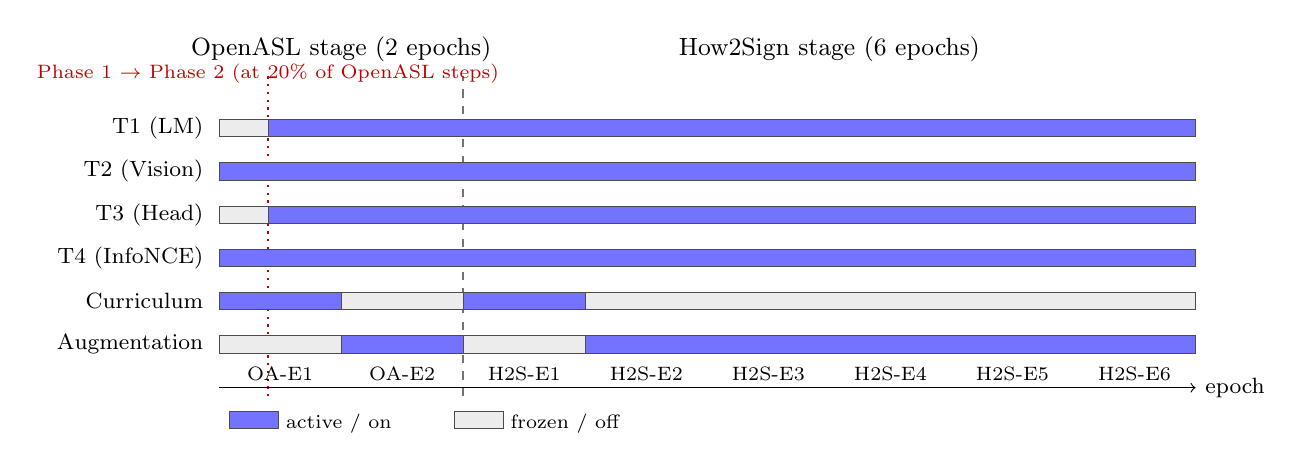
\begin{tikzpicture}[
  x=1.55cm, y=0.55cm,
  on/.style={fill=blue!55,  draw=black!70, very thin},
  off/.style={fill=gray!15, draw=black!70, very thin},
  rowlabel/.style={font=\footnotesize, anchor=east},
  epochlabel/.style={font=\scriptsize, anchor=north},
  stagelabel/.style={font=\small, align=center, anchor=south},
  phasemark/.style={font=\scriptsize, anchor=south, text=red!75!black},
]
% Coordinate system: 1 x-unit = 1 epoch. Total of 8 epochs.
% [0,1]   OpenASL E1     (Phase 1 occupies [0, 0.4], Phase 2 occupies [0.4, 1])
% [1,2]   OpenASL E2     (all Phase 2)
% [2,8]   How2Sign E1..E6 (single phase)
\def\xphase{0.4}     % Phase 1 -> 2 boundary
\def\xstage{2}        % OpenASL -> How2Sign boundary
\def\xend{8}

% Stage headers
\node[stagelabel] at (1,   6.5) {OpenASL stage (2 epochs)};
\node[stagelabel] at (5,   6.5) {How2Sign stage (6 epochs)};

% Stage divider
\draw[dashed, black!55, thick] (\xstage, -1.0) -- (\xstage, 6.4);

% Phase 1 -> Phase 2 marker
\draw[dotted, red!75!black, thick] (\xphase, -1.0) -- (\xphase, 6.4);
\node[phasemark] at (\xphase, 6.0) {Phase 1 $\to$ Phase 2 (at 20\% of OpenASL steps)};

% ─── Tier rows ─────────────────────────────────────────────────────────────
\node[rowlabel] at (-0.05, 5.2) {T1 (LM)};
\fill[off] (0,       5.0) rectangle (\xphase, 5.4);
\fill[on]  (\xphase, 5.0) rectangle (\xend,   5.4);

\node[rowlabel] at (-0.05, 4.2) {T2 (Vision)};
\fill[on] (0, 4.0) rectangle (\xend, 4.4);

\node[rowlabel] at (-0.05, 3.2) {T3 (Head)};
\fill[off] (0,       3.0) rectangle (\xphase, 3.4);
\fill[on]  (\xphase, 3.0) rectangle (\xend,   3.4);

\node[rowlabel] at (-0.05, 2.2) {T4 (InfoNCE)};
\fill[on] (0, 2.0) rectangle (\xend, 2.4);

% ─── Curriculum row ───────────────────────────────────────────────────────
% Curriculum ON during E1 of each stage: x in [0,1] (OA E1) and [2,3] (H2S E1).
\node[rowlabel] at (-0.05, 1.2) {Curriculum};
\fill[on]  (0, 1.0) rectangle (1,      1.4);
\fill[off] (1, 1.0) rectangle (\xstage, 1.4);
\fill[on]  (\xstage, 1.0) rectangle (3, 1.4);
\fill[off] (3, 1.0) rectangle (\xend,  1.4);

% ─── Augmentation row ─────────────────────────────────────────────────────
% Augmentation OFF during E1 of each stage, ON from E2 onward.
\node[rowlabel] at (-0.05, 0.2) {Augmentation};
\fill[off] (0,       0.0) rectangle (1,      0.4);
\fill[on]  (1,       0.0) rectangle (\xstage, 0.4);
\fill[off] (\xstage, 0.0) rectangle (3,      0.4);
\fill[on]  (3,       0.0) rectangle (\xend,   0.4);

% ─── Epoch tick labels ────────────────────────────────────────────────────
\node[epochlabel] at (0.5, -0.1) {OA-E1};
\node[epochlabel] at (1.5, -0.1) {OA-E2};
\node[epochlabel] at (2.5, -0.1) {H2S-E1};
\node[epochlabel] at (3.5, -0.1) {H2S-E2};
\node[epochlabel] at (4.5, -0.1) {H2S-E3};
\node[epochlabel] at (5.5, -0.1) {H2S-E4};
\node[epochlabel] at (6.5, -0.1) {H2S-E5};
\node[epochlabel] at (7.5, -0.1) {H2S-E6};

% Time axis
\draw[->, thin] (0, -0.8) -- (\xend, -0.8) node[right, font=\footnotesize] {epoch};

% ─── Legend ───────────────────────────────────────────────────────────────
\node[anchor=west, font=\scriptsize] at (0, -1.6)
    {\tikz\fill[on]  (0,0) rectangle (0.4,0.4); active / on
     \hspace{0.6cm}
     \tikz\fill[off] (0,0) rectangle (0.4,0.4); frozen / off};

\end{tikzpicture}
\caption{Training schedule over the eight training epochs. For each tier
(T1--T4), the bar indicates whether the tier is receiving gradient updates
(filled) or frozen (grey). The bottom two rows show whether the easy-first
curriculum and the stochastic augmentation suite are active. T2 and T4 are
active from the first optimiser step; T1 and T3 wake up at the Phase~1 to
Phase~2 boundary inside the OpenASL stage and remain active for the rest of
training. The curriculum is applied only during the first within-stage
epoch of each stage. Augmentation is the opposite: off during the first
within-stage epoch and on from the second epoch onward.}
\label{fig:tier-timeline}
\end{figure}

\subsection{Loss Composition}
\label{sec:train-loss}

The training objective is the sum of two terms. The primary term is the
standard next-token cross-entropy loss between the model's predicted
distribution and the reference English sentence, computed with label
smoothing of $0.04$ to soften the target distribution against the noisier
OpenASL captions. The auxiliary term is an InfoNCE contrastive loss that
encourages the pooled vision embedding of a clip to be closer to the pooled
embedding of its matching reference caption than to the embeddings of
non-matching captions in the same effective batch. Concretely, let $v_i$
and $t_i$ denote the $\ell_2$-normalised projection-head embeddings
(Section~\ref{sec:arch-infonce-heads}) of clip $i$ and its caption, and let
$\tau = 0.07$ be the temperature. The video-to-text direction of the
InfoNCE loss is
\[
\mathcal{L}_{v \to t} = -\frac{1}{N} \sum_{i=1}^{N}
\log \frac{\exp(v_i^\top t_i / \tau)}
         {\sum_{j} \exp(v_i^\top t_j / \tau)},
\]
and the text-to-video direction is defined symmetrically. The negative pool
for $t_j$ includes the current batch and a MoCo-style queue of $64$
recently-seen detached caption embeddings, giving stronger contrastive
pressure than the batch alone provides. The combined loss is
$\mathcal{L} = \mathcal{L}_{\text{CE}} + \lambda \,
(\mathcal{L}_{v \to t} + \mathcal{L}_{t \to v}) / 2$, with
$\lambda = 0.3$ throughout, linearly warmed up over the first $200$ steps to
prevent gradient explosions from the freshly initialised projection heads.

\subsection{Optimiser and Per-Tier Learning-Rate Schedules}
\label{sec:train-optim}

The optimiser is AdamW with $\beta = (0.9, 0.98)$ and a weight decay of
$0.01$, using the 8-bit AdamW implementation to reduce optimiser-state
memory. Each tier owns an independent peak and floor learning rate per
stage, summarised in Table~\ref{tab:lr-schedule}. A shared linear warmup
ratio of $5\%$ of each tier's active step count is followed by cosine decay
to the floor. Tiers 1 and 3 have a smaller active step count than tiers 2
and 4 in the OpenASL stage because their warmup begins at the Phase 1 to
Phase 2 boundary rather than at step zero. The How2Sign-stage peak learning
rates are set systematically below their OpenASL counterparts so that the
fine-tuning stage refines rather than overwrites the OpenASL solution.

\begin{table}[h]
\centering
\caption{Per-tier peak and floor learning rates per training stage. All
tiers use a $5\%$ linear warmup followed by cosine decay.}
\label{tab:lr-schedule}
\begin{tabular}{l l l l l}
\toprule
       & \multicolumn{2}{c}{OpenASL stage} & \multicolumn{2}{c}{How2Sign stage} \\
\cmidrule(lr){2-3} \cmidrule(lr){4-5}
Tier   & Peak LR     & Floor LR        & Peak LR     & Floor LR        \\
\midrule
T1     & $3 \times 10^{-5}$ & $1.5 \times 10^{-6}$ & $2 \times 10^{-5}$ & $5 \times 10^{-7}$ \\
T2     & $5 \times 10^{-5}$ & $2.5 \times 10^{-6}$ & $4 \times 10^{-5}$ & $2 \times 10^{-6}$ \\
T3     & $2 \times 10^{-5}$ & $1 \times 10^{-6}$   & $1 \times 10^{-5}$ & $5 \times 10^{-7}$ \\
T4     & $5 \times 10^{-5}$ & $2.5 \times 10^{-6}$ & $3 \times 10^{-5}$ & $1.5 \times 10^{-6}$ \\
\bottomrule
\end{tabular}
\end{table}

\subsection{Per-Tier Gradient Clipping}
\label{sec:train-clip}

Each tier is clipped independently rather than under a single global norm,
so that a high-norm tier (typically T2, the vision encoder) cannot drag
down the gradients of well-behaved tiers. The clipping thresholds are
$5.0$ for T1, $9.0$ for T2 (a more generous limit reflecting the
naturally larger gradient magnitudes of the vision adapters), $3.0$ for
T3, and $2.0$ for T4. The joint global gradient norm is still computed and
logged for diagnostics but is not used to clip.

\subsection{Checkpointing, Resume, and Early Stopping}
\label{sec:train-ckpt}

Checkpoints are written every $10$ optimiser steps, retaining the eight
most recent. Each checkpoint contains the LoRA adapter weights, the
InfoNCE projection-head weights, the per-tier optimiser and scheduler
states, the InfoNCE queue contents, and all random-number generator states
required for a bit-faithful resume modulo the inherently nondeterministic
augmentation and dropout sources. Validation runs every $80$ optimiser
steps, and early stopping is applied.


\section{Engineering and Infrastructure}
\label{sec:engineering}

\subsection{Compute Environment and Training Cost}
\label{sec:eng-compute}

Training was carried out on a single NVIDIA A100 GPU with $80$ GB of memory,
rented from a cloud GPU provider. The effective batch size was $24$, formed
from a per-device micro-batch of $6$ samples and $4$ gradient-accumulation
steps. The OpenASL stage ran for $2{,}448$ optimiser steps and the How2Sign
stage ran for $3{,}540$ optimiser steps, giving $5{,}988$ optimiser steps in
total. The complete training run took $4$ days and $18$ hours.

\subsection{Memory and Throughput Optimisations}
\label{sec:eng-mem}

Several memory and throughput optimisations were required to fit the model
and its training state within $80$ GB of GPU memory. Model weights and
activations are kept in bfloat16. Attention is computed with FlashAttention
2, which avoids materialising the full attention matrix and reduces both
compute and memory cost. Gradient checkpointing trades activation
recomputation for further memory savings. The optimiser state is held in
8-bit AdamW, which reduces memory footprint relative to standard
32-bit AdamW. Liger fused Triton kernels are used to reduce memory and accelerate the
forward and backward passes. The PyTorch caching allocator
is configured with \texttt{expandable\_segments:True} to limit fragmentation
across batches of variable-length video. On the input side, the DataLoader
uses eight persistent worker processes with a prefetch factor of six and
pinned host memory, so that video decoding and CPU-side preprocessing
overlap with GPU compute.


\section{Evaluation Protocol}
\label{sec:evaluation}

\subsection{Metrics}
\label{sec:eval-metrics}

The primary text-similarity metric is corpus-level BLEU-4, computed with the
\texttt{sacrebleu} reference implementation. Three additional metrics are
reported alongside BLEU. ROUGE-L is the longest-common-subsequence-based
F-score between predicted and reference sentences. METEOR is the unigram
F-score with stemming and synonym bonuses, computed using NLTK. Word Error
Rate (WER) is the corpus-level Levenshtein edit distance between predicted
and reference word sequences, divided by the total reference word count and
expressed as a percentage. A distinct-$2$ diversity ratio (number of unique
bigrams in the model's generations divided by the total number of generated
bigrams) is also tracked as a simple check against output collapse onto a
small set of fluent but generic phrases. Independently of the generation
metrics, the standard next-token cross-entropy loss and its corresponding
perplexity are reported on the held-out captions.

\subsection{Generation Configuration}
\label{sec:eval-gen}

Predicted translations are produced by beam search with a beam size of $5$,
a length penalty of $0.6$, a no-repeat-$n$-gram constraint of $n = 4$, and a
repetition penalty of $1.1$, and are limited to at most $32$ newly generated
tokens. The no-repeat-$n$-gram constraint and the repetition penalty were
chosen to suppress the short pathological loops (such as repeated
punctuation or repeating stock phrases) observed in early generations.

\section{Results}
\label{sec:results}

All results reported in this section are from the checkpoint at global step $4{,}610$,
selected on the basis of validation loss. Evaluation is performed on the held-out
test set for the How2Sign source ($944$ clips); the OpenASL test partition was
excluded from generation evaluation because no comparable reference translations
were retained after cleaning.

\subsection{Training Dynamics}
\label{sec:results-dynamics}

Figure~\ref{fig:loss-curve} shows the training and validation cross-entropy loss
over the full $5{,}988$ optimiser steps. The OpenASL stage occupies steps $1$
to $2{,}448$ and the How2Sign stage occupies steps $2{,}449$ to $5{,}988$.
Training loss decreases steadily throughout the OpenASL stage. At the
transition to How2Sign, both curves briefly spike before resuming their
downward trend, consistent with a cosine schedule reset and a shift in data
distribution. By the end of How2Sign training the validation loss is stable
at approximately $2.8$.

\begin{figure}[H]
  \centering
  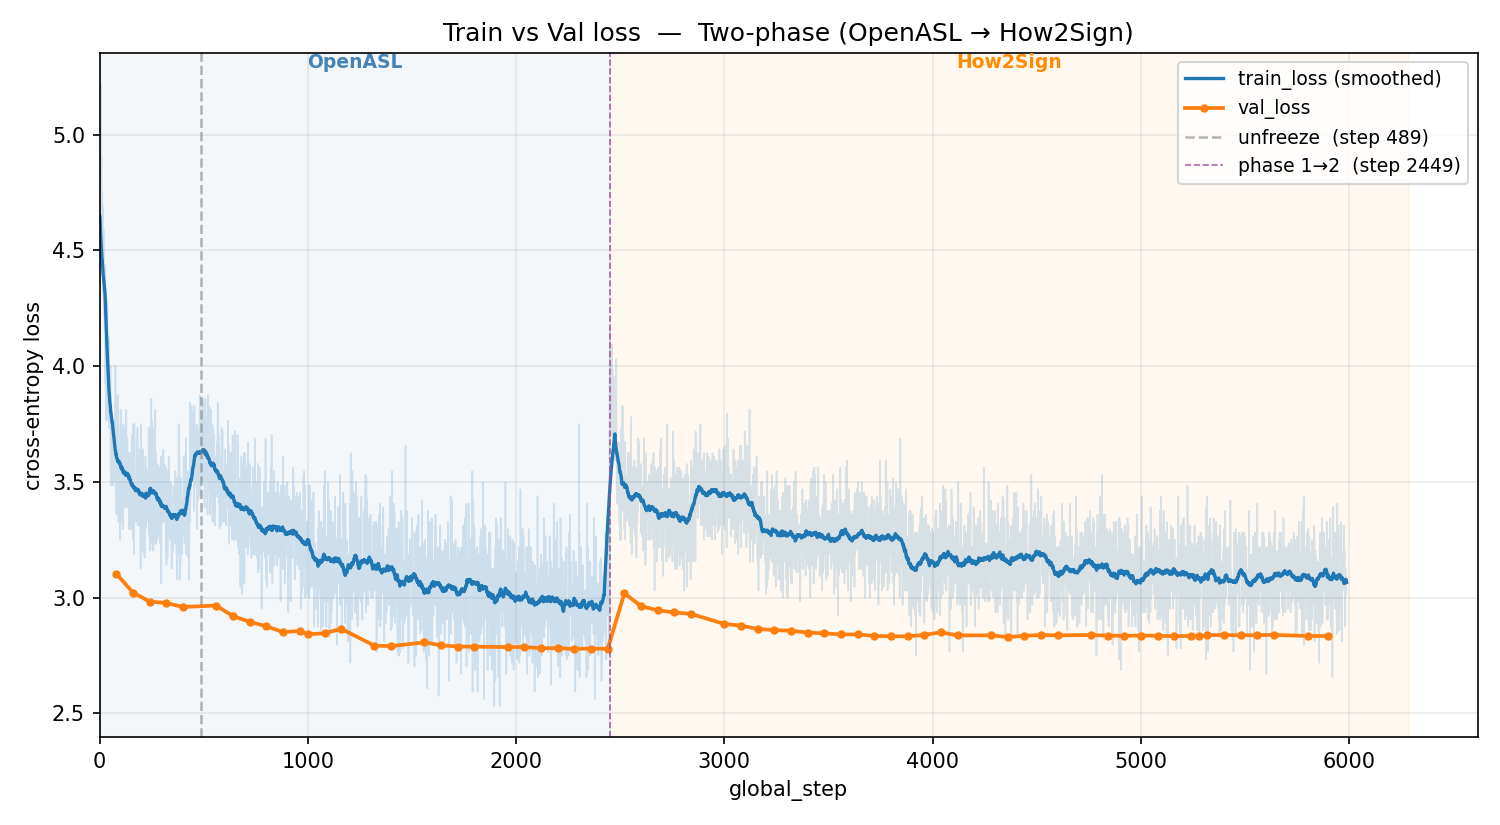
\includegraphics[width=0.92\linewidth]{loss.png}
  \caption{Training and validation cross-entropy loss over the full two-stage
  training run. The dashed vertical lines mark the Phase~1 to Phase~2
  boundary inside the OpenASL stage (step $489$) and the OpenASL to
  How2Sign stage boundary (step $2{,}449$).}
  \label{fig:loss-curve}
\end{figure}

\subsection{Generation Metrics over Training}
\label{sec:results-gen-dynamics}

Figure~\ref{fig:gen-metrics} shows BLEU-1, BLEU-2, BLEU-4, and ROUGE-L on the
How2Sign and OpenASL validation sets, reported at each validation step.
Metrics on both sources improve gradually through the OpenASL stage and
accelerate visibly once How2Sign fine-tuning begins at step $2{,}449$, at
which point the How2Sign curves (blue) rise sharply while the OpenASL
curves (orange) plateau. This behaviour confirms that the staged schedule
achieves its intended effect: OpenASL pretraining moves the model into the
signing domain, while How2Sign fine-tuning sharpens it on the
higher-quality target distribution.

\begin{figure}[H]
  \centering
  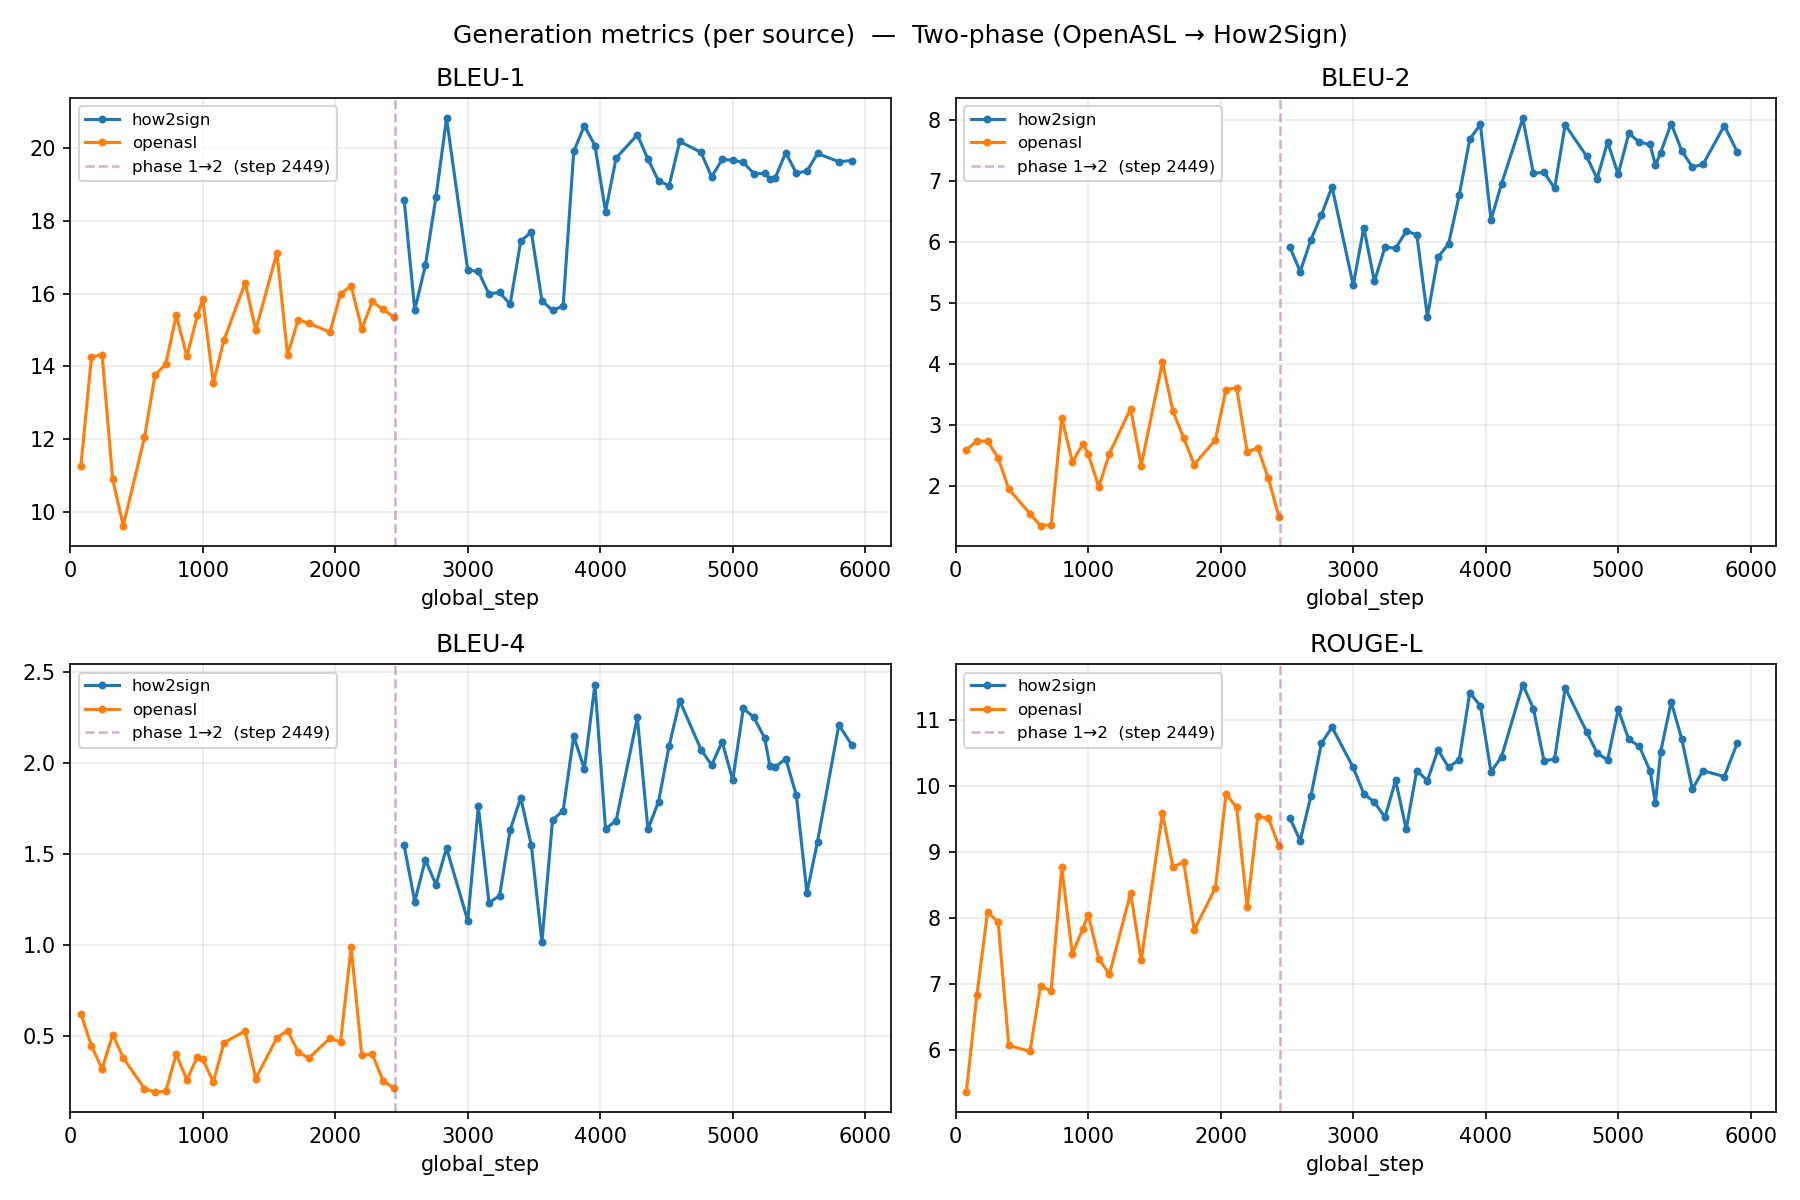
\includegraphics[width=0.92\linewidth]{gen_metrics_bleu_rouge.png}
  \caption{Validation BLEU-1, BLEU-2, BLEU-4, and ROUGE-L over training,
  plotted per source (How2Sign = blue, OpenASL = orange). The dashed
  vertical line at step $2{,}449$ marks the OpenASL to How2Sign stage
  boundary.}
  \label{fig:gen-metrics}
\end{figure}

\subsection{Best-Checkpoint Test Metrics}
\label{sec:results-metrics}

Table~\ref{tab:test-results} summarises the generation and loss metrics on
the How2Sign test set at the selected checkpoint.

\begin{table}[H]
\centering
\caption{Test-set results at step $4{,}610$ on the How2Sign test partition
($944$ clips). Loss and perplexity are computed on teacher-forced reference
tokens; all other metrics are computed on beam-search generations.}
\label{tab:test-results}
\begin{tabular}{l r}
\toprule
Metric          & Value   \\
\midrule
Test loss       & $2.7896$ \\
Perplexity      & $16.28$  \\
\midrule
BLEU-1          & $19.76$  \\
BLEU-2          & $6.95$   \\
BLEU-4          & $1.64$   \\
chrF            & $17.42$  \\
ROUGE-L         & $10.43$  \\
METEOR          & $9.71$   \\
WER (\%)        & $112.51$ \\
Distinct-2      & $0.103$  \\
\midrule
Mean ref.\ length (words) & $12.91$ \\
Mean hyp.\ length (words) & $14.39$ \\
\bottomrule
\end{tabular}
\end{table}

The model achieves a BLEU-4 of $1.64$ and a ROUGE-L of $10.43$. These
numbers are relatively low, reflecting the small backbone, the
limited compute budget, and the inherent difficulty of continuous ASL
translation. The word error rate of $112.51\%$ indicates that, while the model
produces fluent English, the specific words generated frequently do not match
the reference exactly. This behaviour is consistent with a WER above $100\%$,
which arises when the hypothesis is longer than the reference and the
overlapping tokens are few. The distinct-2 score of $0.103$ confirms that the
model's output is not collapsed onto a small set of repeated phrases, though
diversity remains limited.

\subsection{Qualitative Examples}
\label{sec:results-qualitative}

Table~\ref{tab:qualitative} shows three good generated predictions
alongside one clear mismatch.

\begin{table}[H]
\centering
\caption{Selected generation examples from the How2Sign test set: three good
generated predictions and one representative mismatch.}
\label{tab:qualitative}
\begin{tabular}{p{0.46\linewidth} p{0.46\linewidth}}
\toprule
Reference & Hypothesis \\
\midrule
``Well, today I'm going to show you how.''
  & ``I'm going to show you how to do that.'' \\[4pt]
``Now with anything, practice makes perfect.''
  & ``I'm going to show you how to do that in the next segment.'' \\[4pt]
``It really just takes some practice.''
  & ``We're going to do the same thing on the other side.'' \\
\midrule
``Don't panic, don't freak out, it's really not difficult.''
  & ``We're going to talk about how to choose a good pair of running shoes.'' \\
\bottomrule
\end{tabular}
\end{table}

The best-matching predictions read as natural, fluent English sentences in
the same instructional style as the references, and in several cases they
capture much of the original meaning, even when the exact wording differs.
The mismatch example is a clearer failure: the reference and the hypothesis
are about completely different things. Together, these cases show that the
model has learned to produce sensible How2Sign-style sentences and can often
get the meaning roughly right, but it is not yet reliable at tying a
specific clip to its specific caption.


\section{Limitations and Lessons Learned}
\label{sec:limitations}

\subsection{Custom Data Split}
\label{sec:lim-split}

The most consequential methodological caveat in this work is the use of a
custom $90/5/5$ stratified split rather than the released How2Sign and
OpenASL splits. The choice was driven by the cleaning passes described in
Section~\ref{sec:data-splits}, which removed exact duplicates, cross-split
near-duplicates, and clips with implausible words-per-second, and left the
official per-split sizes unbalanced enough that pooling and re-splitting the
cleaned data produced a more uniform evaluation set. The cost is that the
numbers reported in Section~\ref{sec:results} cannot be accurately compared
against published results directly.

\subsection{Modest Metrics and High Word Error Rate}
\label{sec:lim-metrics}

As discussed in Section~\ref{sec:results-metrics}, the test-set BLEU-4 of
$1.64$ and word error rate of $112.51\%$ are modest in absolute terms. The
qualitative examples in Section~\ref{sec:results-qualitative} show that the
system is fluent and often captures the meaning of the reference, but the
exact wording frequently differs, which the $n$-gram metrics penalise
heavily. There is therefore still room to improve the alignment between
generated and reference wording before the system is ready for use in
applications that depend on faithful sentence-level translation.

\subsection{Single-GPU Compute Budget}
\label{sec:lim-compute}

All training was performed on a single NVIDIA A100 with $80$ GB of memory.
This budget shaped several decisions: the choice of a $2$-billion-parameter
backbone rather than a larger Qwen3-VL variant, the reliance on LoRA rather
than full fine-tuning, the use of bfloat16 weights, 8-bit AdamW, and
gradient checkpointing, and the cap on per-frame pixel budget. A larger
compute budget would have removed or relaxed each of these constraints.

\subsection{Lessons Learned}
\label{sec:lim-lessons}

Three short takeaways stand out from the project. First, splitting the
trainable parameters into independently-scheduled tiers, rather than
applying a single LoRA configuration across the whole model, made the
training much easier to reason about and tune. Second, staging a noisier,
larger corpus before a cleaner, smaller one produced the clearest
inflection in the generation-metric curves at the stage boundary, which
suggests the staged schedule was working as intended. Third, careful data
cleaning, in particular the removal of cross-split near-duplicates, mattered
more for trustworthy evaluation than any single training-recipe change.


\section{Future Work}
\label{sec:future-work}

Two directions stand out as the most promising next steps for this work.

The first is to repeat the same recipe with a larger vision and language
backbone. The $2$-billion-parameter Qwen3-VL variant used here was chosen
to fit within the available single-GPU budget, but the Qwen3-VL family
also includes substantially larger variants whose stronger language priors
and richer visual representations should help the model produce
translations that match the reference more closely at the word level, not
just at the level of register and topic.

The second is to expand the training pool with additional clean
paired data. The cleaning passes applied in this work removed a noticeable
fraction of the original corpora, and the remaining data is dominated by a
relatively narrow set of signers and recording conditions. Incorporating
further clean ASL-to-English material, whether from larger open corpora or
from carefully curated new sources, would broaden the distribution of
signers, topics, and recording conditions and is likely to improve
generalisation more than any single change to the training recipe.


\section{Conclusion}
\label{sec:conclusion}

This report has documented an end-to-end pipeline for translating continuous
American Sign Language video into English text, built around a fine-tuned
Qwen3-VL-2B-Instruct backbone. The contribution is not a new model or a
state-of-the-art result but a transparent account of one engineering
recipe: a multi-tier LoRA / RSLoRA adaptation, a two-corpus staged
training schedule from the larger and noisier OpenASL corpus to the cleaner
How2Sign corpus, a preprocessing pipeline combining pose-guided signer
cropping, CLAHE contrast enhancement, and pre-extracted MediaPipe landmark
overlays, and an InfoNCE auxiliary loss anchoring the pooled vision
representation to its caption embedding. The resulting system produces
fluent English in the register of the target captions and often captures
the meaning of the signed input, while the word-level overlap with
reference translations remains modest. The methodological caveats discussed
in Section~\ref{sec:limitations}, in particular the custom data split, are
stated openly so that the numbers in Section~\ref{sec:results} are read for
what they are: a single, fully documented data point on what is achievable
with a small open backbone, a single-GPU budget, and the publicly available
ASL-to-English data.


\appendix

\section{Full Hyperparameter Configuration}
\label{app:hyperparams}

Table~\ref{tab:hparams} consolidates the training, optimisation, loss, and
data-handling hyperparameters used in the reported run. Per-tier LoRA ranks
are listed in Table~\ref{tab:lora-tiers} and per-tier learning rates are
listed in Table~\ref{tab:lr-schedule}.

\begin{table}[H]
\centering
\caption{Consolidated training-recipe hyperparameters for the reported run.}
\label{tab:hparams}
\begin{tabular}{l l}
\toprule
Hyperparameter                              & Value \\
\midrule
\multicolumn{2}{l}{\emph{Schedule}} \\
OpenASL stage epochs                        & $2$ \\
How2Sign stage epochs                       & $6$ \\
OpenASL Phase 1 fraction (T1, T3 frozen)    & first $20\%$ of OpenASL steps \\
Per-stage warmup ratio                      & $5\%$ of tier's active steps \\
LR decay shape (post-warmup)                & cosine to floor \\
OpenASL optimiser steps                     & $2{,}448$ \\
How2Sign optimiser steps                    & $3{,}540$ \\
Total optimiser steps                       & $5{,}988$ \\
\midrule
\multicolumn{2}{l}{\emph{Batching}} \\
Per-device micro-batch                      & $6$ \\
Gradient accumulation steps                 & $4$ \\
Effective batch size                        & $24$ \\
Bucket batching                             & by clip duration \\
Curriculum (first within-stage epoch only)  & easy-first by clip duration \\
\midrule
\multicolumn{2}{l}{\emph{Optimiser}} \\
Optimiser                                   & 8-bit AdamW \\
$(\beta_1, \beta_2)$                        & $(0.9,\, 0.98)$ \\
Weight decay                                & $0.01$ \\
Per-tier gradient-clipping norm (T1/T2/T3/T4) & $5.0 / 9.0 / 3.0 / 2.0$ \\
\midrule
\multicolumn{2}{l}{\emph{Loss}} \\
Label smoothing                             & $0.04$ \\
InfoNCE weight $\lambda$                    & $0.3$ \\
InfoNCE warmup                              & $200$ steps (linear) \\
InfoNCE temperature $\tau$                  & $0.07$ \\
InfoNCE MoCo queue size                     & $64$ \\
Projection-head dimension                   & $256$ \\
\midrule
\multicolumn{2}{l}{\emph{Video / vision}} \\
OpenASL fps                                 & $18$ \\
How2Sign fps                                & $20$ \\
OpenASL per-frame-pair pixel budget         & $150 \times 32 \times 32 \approx 392{\times}392$ \\
How2Sign per-frame-pair pixel budget        & $180 \times 32 \times 32 \approx 429{\times}429$ \\
Per-clip pixel cap                          & $20{,}480 \times 32 \times 32$ \\
CLAHE clip limit, tile grid                 & $2.0$, $8 \times 8$ (L channel, LAB) \\
\midrule
\multicolumn{2}{l}{\emph{Validation and checkpointing}} \\
Validation cadence                          & every $80$ optimiser steps \\
Checkpoint cadence                          & every $10$ optimiser steps \\
Retained checkpoints                        & $8$ most recent \\
Early stopping                              & enabled \\
\bottomrule
\end{tabular}
\end{table}


\section{Augmentation Parameters}
\label{app:augmentation}

Table~\ref{tab:aug} lists the configuration of the stochastic augmentation
suite referenced in Section~\ref{sec:pre-aug}. All augmentations are
applied per clip, after the three always-on preprocessing stages, and only
when augmentation is enabled (from the second within-stage epoch of each
stage onward). The augmentations listed as \emph{disabled} are present in
the codebase but were turned off for the reported run.

\begin{table}[H]
\centering
\caption{Stochastic augmentation suite. Probabilities are per clip.}
\label{tab:aug}
\begin{tabular}{l l l}
\toprule
Augmentation       & Probability & Parameters \\
\midrule
Temporal jitter    & $0.40$ & shift up to $\pm 2$ frames, edge replication \\
Colour jitter      & $0.40$ & brightness $\pm 0.1$, contrast $\pm 0.1$, saturation $\pm 0.1$, hue $\pm 0.1$ \\
Random grayscale   & $0.07$ & --- \\
Affine             & $0.25$ & rotation $\pm 2^\circ$, translate $\pm 5\%$, scale $0.95$--$1.00$ \\
Speed perturbation & $0.15$ & resample rate $0.9$--$1.0\times$ \\
\midrule
Gaussian blur      & disabled & --- \\
Solarise           & disabled & --- \\
Random erasing     & disabled & --- \\
Histogram equalise & disabled & (replaced by always-on CLAHE) \\
\bottomrule
\end{tabular}
\end{table}


\bibliographystyle{ieeetr}
\bibliography{references}


\end{document}
